\documentclass[12pt]{article}

\usepackage[utf8]{inputenc}
\usepackage[margin = 1in]{geometry}
\usepackage[english]{babel}
\usepackage{amsthm}
\usepackage{amssymb}
\usepackage{amsmath}
\usepackage{changepage}
\usepackage[makeindex]{imakeidx}
\usepackage{titlesec}
\usepackage{textcomp}
\usepackage{gensymb}
\usepackage{xcolor, soul}
\usepackage{hyperref}
\usepackage{pgfplots}
\usepackage{parskip}

\definecolor{linkColour}{RGB}{140, 25, 57}
\definecolor{urlColour}{RGB}{137, 62, 27}

\setcounter{section}{-1}
\setcounter{secnumdepth}{4}

\titleformat{\paragraph}
{\normalfont\normalsize\bfseries}{\theparagraph}{1em}{}
\titlespacing*{\paragraph}
{0pt}{3.25ex plus 1ex minus .2ex}{1.5ex plus .2ex}

\hypersetup{
    colorlinks,
    citecolor=purple,
    filecolor=purple,
    linkcolor=linkColour,
    urlcolor=urlColour
}

\makeindex

\newcommand{\homl}{\hyperlink{homl}{Hands-On Machine Learning}}

\newenvironment{fact*}[2][]
    {
    \begin{adjustwidth}{1em}{0em}
    \noindent
    \textbf{#2} \hfill #1
    
    \vspace{0.1in}
    \noindent
    \ignorespaces
    }
    {
    \end{adjustwidth}
    }

\newenvironment{fact}[2][]
    {
    \index{#2}
    \hypertarget{#2}{\vspace{0.2in}}
    \begin{adjustwidth}{1em}{0em}
    \noindent
    \textbf{#2} \hfill #1
    
    \vspace{0.1in}
    \noindent
    \ignorespaces
    }
    {
    \end{adjustwidth}
    }

\title{Companion to Machine Learning}
\author{Rohan Kumar}
\date{}






\begin{document}

\maketitle
\newpage
\tableofcontents
\newpage

\section*{Sources}
    Throughout this compendium, each piece of information will be formatted as such.
    
    \vspace{0.1in}
    \begin{fact*}[Source]{Name / Description of fact}
        Information about fact.
    \end{fact*}
    \vspace{0.3in}
    
    \noindent The location which currently contains ``Source'' could potentially be filled with a variety of sources. Here is how to find the source based off the shortened form.
    
    \begin{itemize}
        \item \hypertarget{homl}{\textbf{Hands-On Machine Learning}} refers to Hands-On Machine Learning with Scikit-Learn, Keras, and TensorFlow, 2nd Edition by Aurélien Géron
    \end{itemize}

\newpage

\section{Notation}
    \subsection{Data}
    \begin{flalign*}
        \boldsymbol{x} &= \begin{pmatrix} x_1 \\ x_2 \\ ... \\ x_M \end{pmatrix} \text{: data point corresponding to a column vector of $M$ features} & \\
        \overline{\boldsymbol{x}} &= \begin{pmatrix} 1 \\ x_1 \\ x_2 \\ ... \\ x_M \end{pmatrix} \text{: concatenation of 1 with the vector} \boldsymbol{x} & \\
        \boldsymbol{X} &= \begin{pmatrix} x_{1,1} & ... & x_{1,N} \\ ... & ... & ... \\ x_{M,1} & ... & x_{M,N} \end{pmatrix} \text{: dataset consisting of $N$ data points and $M$ features} & \\
        \overline{\boldsymbol{X}} &= \begin{pmatrix} 1 & ... & 1 \\ x_{1,1} & ... & x_{1,N} \\ ... & ... & ... \\ x_{M,1} & ... & x_{M,N} \end{pmatrix} \text{: concatenation of a vector of 1's with the matrix } \boldsymbol{X} & \\
        y &= \text{: output target (regression) or label (classification)} & \\
        \boldsymbol{y} &= \begin{pmatrix} y_1 \\ y_2 \\ ... \\ y_N \end{pmatrix} \text{: vector of outputs for a dataset of $N$ points} & \\
        \boldsymbol{x}_* &= \text{: test input / unknown input } & \\
        \boldsymbol{y}_* &= \text{: predicted output} & \\
        N &= \text{: Number of data points in the dataset} & \\
        M &= \text{: Number of a features in a data point} & \\
        \boldsymbol{w} &= \begin{pmatrix}
            w_1 \\
            w_2 \\
            ... \\
            w_M \\
        \end{pmatrix} & \\
        \boldsymbol{w}^T &= (w_1, w_2, ..., w_M) \text{ or } (w_0, w_1, w_2, ..., w_M) \text{ $w_0$ multiplies the first entry of $\overline{\boldsymbol{x}}$ (bias)} & \\
    \end{flalign*}
    Note: bold symbols represents a vector

\section{Introduction}

\subsection{What is Machine Learning}
    Machine Learning is the field of study that gives computers the ability to learn from data without being 
    explicitly programmed. This is good for problems that require a lot of fine-tuning or for which using a 
    traditional approach yields no good solution. Machine Learning's data dependency allows it to adapt to new data
    and gain insight for complex problems and large amounts of data.

\subsection{Applications of Machine Learning}
    Machine Learning can be used for a range of tasks and can be seen used in:
    \begin{itemize}
        \item Analyzing images of products on a production line to automatically classify them (Convolutional Neural Net)
        \item Forecasting company revenue based on performance metrics (Regression or Neural Net)
        \item Automatically classifying news articles (NLP using Recurrent Neural Networks)
        \item Summarizing long documents automatically (Natural Language Processing)
        \item Building intelligent bot for a game (Reinforcement Learning)
    \end{itemize}

\subsection{Types of Machine Learning}
    \subsubsection{Supervised Learning}
        In supervised learning, the training set you feed to the algorithm includes the desired solutions, called labels.
        (e.g determining if an email is spam would be trained a dataset of example emails labelled as spam or not spam.) \\[0.1in] 
        Some commonly used supervised learning algorithms are:
        \begin{itemize}
            \item k-Nearest Neighbors
            \item Linear Regression
            \item Logistic Regression
            \item Support Vector Machines (SVMs)
            \item Decision Trees and Random Forests
            \item Neural Networks
        \end{itemize}
    
    \subsubsection{Unsupervised Learning}
        In unsupervised learning, the training data is unlabeled and the system tries to learn without guidance. The system
        will try and automatically draw inferences and conclusions about the data and group it as such. (e.g. having a lot of
        data about blog visitors. Using a clustering algorithm we can group and detect similar visitors). \\[0.1in]
        Some important unsupervised learning algorithms are:
        \begin{itemize}
            \item Clustering
            \begin{itemize}
                \item K-Means
                \item DBSCAN
                \item Hierarchical Cluster Analysis
            \end{itemize}
            \item Anomaly detection and novelty detection
            \begin{itemize}
                \item One-class SVM
                \item Isolation Forest
            \end{itemize}
            \item Visualization and dimensionality reduction
            \begin{itemize}
                \item Principal Component Analysis (PCA)
                \item Kernel PCA
                \item Locally Linear Embedding (LLE)
                \item t-Distributed Stochastic Neighbor Embedding (t-SNE)
            \end{itemize}
            \item Association rule learning
            \begin{itemize}
                \item Apriori
                \item Eclat
            \end{itemize}
        \end{itemize}

    \subsubsection{Semisupervised Learning}
        Labelling can be very time-consuming and costly, often there will be plenty of unlabelled and a few labelled instances.
        Algorithms that deal with data that is partially labeled is called semi-supervised learning. A good example of this is
        Google Photos. Google clusters and groups your photos based on facial recognition (unsupervised) and then you can label one photo and it
        will be able to label every picture like that (supervised). Most semi-supervised learning algorithms are combinations of unsupervised and 
        supervised algorithms.  
    
    \subsubsection{Reinforcement Learning}
        Reinforcement Learning is a learning algorithm based on a reward system. The learning system, called an agent, can observe the environment,
        select and perform actions, and get rewards in return (or penalties in the form of negative rewards). It will then learn by itself what the 
        best strategy, called a policy, to get the most reward over time. A policy defines what action the agent should choose when it is in a given
        situation.

\section{Data Analysis}
    \subsection{Limitations of Data}
        \subsubsection{Nonrepresentative Training Data}
        One thing to look out for when using training data is whether the data is 
        representative of the new cases you want to generalize to. For example if you are training linear regression life satisfaction vs GDP of countries,
        if some countries are missing from the dataset then the dataset is not fully representative of the problem.

        \subsubsection{Poor Quality Data}
        If your data is full of errors, outliers and noise, it will make it harder for the system to detect the underlying patterns, so your system is less likely
        to perform well. In order to mitigate this we need to clean the training data.
        \begin{itemize}
            \item If some instances are outliers, it may help to discard them or try to fix the errors manually
            \item If some instances are missing features, you may decide to ignore that attribute, ignore the instance, fill in the missing values, or train one model with the feature and one without
        \end{itemize}

        \subsubsection{Irrelevant Features}
        A critical part of the success of a Machine Learning project is coming up with a good set of features to train on. This process is called \textit{feature engineering}.
        \begin{itemize}
            \item \textit{Feature selection}: Selecting the most useful features to train on among the existing features
            \item \textit{Feature extraction}: Combining existing features to produce a more useful one (dimensionality reduction algorithms can help)
            \item Creating new features by gathering new data.
        \end{itemize}

    \subsection{Feature Engineering}
        \subsubsection{Feature Construction}
            Features can be modified for various reasons, including to increase predictor performance and to reduce time or memory requirements.
            Below are common techniques for constructing features.

            \paragraph{Transformation}
            Common feature transformations include:
            \begin{itemize}
                \item \textbf{Centering} each feature to be around the origin.
                \item \textbf{Scaling} each feature to be of the same scale. For example, scaling can be done to make sure each feature has the same
                variance or the same maximum absolute value.
                \item \textbf{Logarithmically} transforming each feature to reduce the skewness of feature distributions.
            \end{itemize}

            Note that feature transformation runs the risk of discarding useful information. For example, scaling to make each feature have the same
            variance should not be done if the differing variances of the features are actually relevant to the problem.

            \paragraph{Feature Extraction}
            Feature expansion involves combining multiple features into new features when first order interactions are not good enough. For example, given
            features $x_1$ and $x_2$, $x_1 \cdot x_2$ is a new feature (i.e. meta-feature) formed by an expansion of $x_1$ and $x_2$.

            \paragraph{``Ad hoc'' Features}
            Constructing ad hoc features involves applying domain knowledge to introduce custom features.

        \subsubsection{Feature Selection}
            Irrelevant features are features that are uncorrelated with a prediction task. Redundant features are features that are highly correlated with
            one another, so using multiple redundant features does not help with predictions much more than using a single such feature.

            Different learning algorithms have differing levels of robustness to irrelevant or redundant features. For example, decision trees are robust
            to redundant features, since such features have low information gain, while KNN is not, since the set of redundant features will behave as one heavily
            weighted feature. When possible, these feature should not be selected in the first place. Below are common ways to avoid selecting such features.

            \paragraph{Wrapper Methods}
            Wrapper methods involve building a model for feature subsets, and then selecting the best performing model. A ``forward search'' approach
            starts with no features and then adds the feature that best improves the model until a certain number of features are selected.  A
            ``backward'' search approach starts with all features and removes the feature that improves the model the least until a certain number
            of features have been removed.

            Computing all possible feature subsets would guarantee finding the optimal one. However, a problem with $M$ features has $2^M$ possible
            feature subsets, so finding all possible subsets is infeasible for large values of $M$. The forward and backward search approaches
            approximate this but with a time complexity of $O(M^2)$.

            \paragraph{Filter Methods}
            Filter methods, also known as variable ranking, involve assigning each feature a score measuring how informative it is in predictions. This
            score is determined by some ``scoring function'' $S$. Features are then ranked by score, and a number of top features are selected.

            \paragraph{Embedded Methods}
            Embedded methods involve  modifying the cost function to constrain the choice of model. A common example of this is regularization, which can
            be used to penalize complex models and encourage a sparse feature set.

    \subsection{Overfitting}
        \textit{Overfitting} is when the model performs well on the training data, but does not generalize well. Complex models can detect subtle patterns in the data,
        but if the training set is noise, or if it is too small, then the model will likely detect patterns in the noise itself. These patterns will not generalize to
        new instances. Overfitting often happens when the training data has many features, which allows for an approximation of the target function with many degrees of freedom.
        We can use regularization to constrain a model to make it simpler to reduce the risk of overfitting.

    \subsection{Underfitting}
        \textit{Underfitting} is the opposite of overfitting: it occurs when the model is too simple to learn the underlying structure of the data. Methods of fixing the problem include:
        \begin{itemize}
            \item Select a more powerful model, with more parameters.
            \item Feed better features to the learning algorithm
            \item Reduce the constraints on the model (e.g., reduce the regularization hyperparameter)
        \end{itemize}

    \subsection{Bias Variance Decomposition}
        Many machine learning algorithms are based on building a formal model based on the training data (e.g. a decision tree). Models have
        parameters, which are characteristics that can help in classification (e.g. a node in a decision tree). Models may also have hyper-parameters,
        which in turn control other parameters in a model (e.g. max height of decision tree).

        Generalization errors result from a combination of noise, variance, and bias. Bias concerns how well the type of model fits the data. Models
        with high bias pay little attention to training data and suffer from underfitting, while models with low bias may pay too much attention to
        training data and become overfitted. Bias and variance tend to be at odds with one another (high bias typically leads to low variance, and vice
        versa).

\section{Evaluation of Learning}
    \subsection{Performance Formulation}
        Let $y_*$ be an output generated by a function $f$ approximating some target function. Let $y$ be the corresponding
        output of the target function. A loss function $l(y, y_*)$ can be used to measure the accuracy of the approximation
        function $f$. Some common loss functions include:
        \begin{itemize}
            \item Squared Loss: $l(y, y_*) = (y - y_*)^2$
            \item Absolute Loss: $l(y, y_*) = |y - y_*|$
            \item Zero/One Loss: $l(y, y_*) = 1_{y \neq y_*}$
        \end{itemize}

        We assume that the data coming from our target function comes from some probability distribution $D$, and that our training data
        is a random sample of $(x, y)$ pairs from $D$. A Bayes Optimal Classifier is a classifier that for any input $x$, returns the
        $y$ most likely to be generated by $D$.

        Based on the available training data, the goal of supervised learning is to find a mapping $f$ from $x$ to $y$ such that
        generalization error $\sum_{(x,y)} D(x,y)l(y,f(x))$ is minimized. However, since $D$ is unknown, we instead estimate the error from
        the average error in our training or test data, which is $\frac{1}{N}\sum_{n=1}^N l(y_n, f(x_n))$.

    \subsection{Testing and Validation}
        Models are initially built based on a training dataset. Test sets (also known as holdout sets) are then used to estimate the generalization
        error. Validation sets are also used to measure the model's performance, but unlike test sets, validation sets can make changes to the model's
        parameters.

        \subsubsection{Cross Validation}
            Cross validation is a technique for measuring how well a model generalizes. The idea behind it is to break up a training data set into $K$
            equally sized partitions, and use $K-1$ of the partitions as training data and the remaining partition for testing. This should be repeated
            $K$ times, so that all points of data are at some point used for testing. Higher values of $K$ lower the amount of variance of in the error
            estimation. To avoid training and testing data having a different probability distribution, the data should be shuffled before being split.
        \subsubsection{Bootstrapping}
            Bootstrapping is an alternative to cross validation where instead of dividing a training data set into partitions, a random sample of points
            (with possible duplicates) is used as training data. The remaining points are then used as testing data, with the goal being similar to
            that of cross validation.
    
    \subsection{Performance Evaluation of Classifiers}
        Consider the following terminology for classification problems:
        \begin{itemize}
            \item True positive ($TP$) - Examples of class 1 predicted as class 1
            \item False positive ($FP$) - Examples of class 0 predicted as class 1 (Type 1 Error)
            \item True negative ($TN$) - Examples of class 0 predicted as class 0
            \item False negative ($FN$) - Examples of class 1 predicted as class 0 (Type 2 Error)
        \end{itemize}
    
        \subsubsection{Accuracy and Error}
            The following formulas can be used to measure accuracy and error:
            $$Accuracy = \frac{TP + TN}{TP + TN + FP + FN}$$
            $$ErrorRate = \frac{FP + FN}{TP + TN + FP + FN}$$
    
        \subsubsection{Precision and Recall}
            Precision and recall can be measured as follows:
            $$P = \frac{TP}{TP + FP}$$
            $$R = \frac{TP}{TP + FN}$$
    
            Precision measures the ratio of positive predictions that were correct, while recall measures the ratio of total positive instances that were
            predicted. Similarly to how variance and bias are often at odds with one another, so are precision and recall.
    
        \subsubsection{F-Measure}
            An F-measure (also known as a F1 score) measures a model's accuracy by taking into account both precision and recall as follows:
            $$F = \frac{2PR}{P + R}$$
    
            To adjust the relative importance of precision vs recall, a weighted F-measure can be used, which is defined as follows:
            $$F = \frac{(1 + \beta^2)PR}{\beta^2 P + R}$$
    
            In a standard F-measure, $\beta = 1$, $\beta < 1$ means that precision is valued over recall, while $\beta > 1$ means recall is valued over precision.
    
        \subsubsection{Sensitivity and Specificity}
            Sensitivity is the same measure as recall. Specificity is a measure of how well a classifier avoids false positives, and is measured as:
            $$Specificity = \frac{TN}{TN + FP}$$

\section{Activation Functions}
    \subsection{Sigmoid Function}
        The \textit{sigmoid function} denoted $\sigma(\cdot)$ outputs a number between 0 and 1. It is defined as
        $$ \sigma(t) = \frac{1}{1 + exp(-t)} $$

        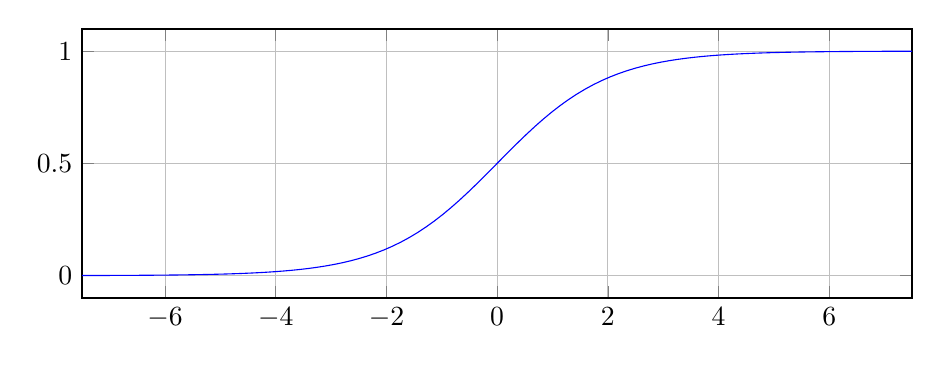
\begin{tikzpicture}
            \begin{axis}
            [%
                axis line style = thick,
                grid=major,
                xmin=-7.5,
                xmax=7.5,
                ytick={0,.5,1},
                width = \linewidth,
                height = 5cm
            ]
                \addplot%
                [
                    blue,%
                    mark=none,
                    samples=100,
                    domain=-7.5:7.5,
                ]
                (x,{1/(1+exp(-x))});
            \end{axis}
        \end{tikzpicture}

        The key property of the sigmoid function is that $\sigma(t) < 0.5$ when $t < 0$, and $\sigma(t) \geq 0.5$ when $t \geq 0$, so a sigmoid function is useful for classification since it can predict 1 when $\boldsymbol{w}^T\boldsymbol{x}$
        is positive and 0 if it is negative.

\section{Convex Optimization}
    In machine learning we can often turn problems into convex functions and simplify the problem into finding the global minima of the function, which in essence is minimizing the training error. One of the key theorem's of a convex function is 
    that the local minimum of a convex function is also a global minimum. Therefore we can apply many methods to find parameters that satisfy the global minima.

    \subsection{Normal Solution}
        To find the value of our parameter (generally $\boldsymbol{w}$) that minimizes the cost function, there is a closed-form solution. We can express this closed form solution for any convex loss function as follows.
        $$ \frac{\partial J(\boldsymbol{w})}{\partial \boldsymbol{w}} = 0 $$
        
        The limitations of using the Normal Solution is that we usually have to compute the inverse of $\boldsymbol{X}^T\boldsymbol{X}$ which is a $(M+1) \times (M+1)$ matrix (where $M$ is the number of features). The computational complexity of inverting 
        such a matrix is typically about $O(M^{2.4})$ to $O(M^{3})$, depending on the implementation. Some of the other approaches below are better suited for cases where there are a large number of features or too many training instances
        to fit in memory.

    \subsection{Gradient Descent}
        Gradient Descent is a generic optimization algorithm capable of finding optimal solution to a wide range of problems. The general ida is to tweak parameters iteratively in order to minimize a cost function. The main concept utilized in
        gradient descent is to measure the local gradient of the error with regard to the parameter vector and move in the direction of the descending gradient. Once the gradient is zero, you have reached the minimum.

        You start with filling your parameter $\boldsymbol{w}$ with random values (random initialization. Then you improve it gradually, taking small steps at a time, each step attempting to decrease the cost function, until the algorithm converges
        to a minimum. One important parameter of Gradient Descent is the size of the steps, determined by the \textit{learning rate} hyperparameter. If the learning rate is too small, then the algorithm will have to go through many iterations to converge,
        if the learning rate is too high, you might jump across the minimum possibly, higher than you were before and potentially make the algorithm diverge. One gradient descent technique is having a learning rate that changes as you approach 
        the minimum to prevent overshoot, also called the learning schedule.

        A limitation of Gradient Descent is when the cost function we are dealing with is not a convex function. In this case holes, ridges, irregular terrain will make the convergence to the minimum difficult.

        \subsubsection{Batch Gradient Descent}
            To implement Gradient Descent, you need to compute the gradient of the cost function with regard to each model parameter $w_j$ - how much the cost function will change if you change $w_j$
            a little bit. This is equivalent to the partial derivative of the cost function with regard to the parameter $w_j$. For the entire parameter vector $\boldsymbol{w}$ we can denoted the gradient vector as
            $\nabla_{\boldsymbol{w}} J(\boldsymbol{w})$.

            Once we have the gradient vector, which points uphill, we descend in the opposite direction (subtract $\nabla_{\boldsymbol{w}} J(\boldsymbol{w})$ from $\boldsymbol{w}$). This is where we use our learning rate $\alpha$ to determine the size of the
            downhill step.
            $$ \boldsymbol{w}^{(next step)} = \boldsymbol{w} - \alpha \nabla_{\boldsymbol{w}} J(\boldsymbol{w}) $$

            The limitation of Batch Gradient Descent is the fact that it uses the whole training set to compute the gradients at every step, which makes it very slow when the training set is large.
        
        \subsubsection{Stochastic Gradient Descent}
            Stochastic Gradient Descent picks a random instance in the training set at every step and computes the gradients based on only that single instance. This makes the algorithm much faster and also makes it possible to train on huge training sets.
            However, due to its stochastic nature, this algorithm will bounce up and down, decreasing only on average. Over time it will end up very close to the minimum, but once it gets there it will continue to bounce around, never settling down.
            Therefore, once the algorithm stops, the final parameter values are good, but not optimal.

            This can actually help when the cost function is very irregular (not convex) as it can help the algorithm jump out of a local minima. One solution to the problem of being unable to settle at the minimum 
            is gradually reducing the learning rate. The steps start out large (helps make quick progress and escape local minima), then get smaller and smaller, allowing the algorithm to settle at the global minima.
            The function that determines the learning rate is called the \textit{learning schedule}.
        
        \subsubsection{Mini-batch Gradient Descent}
            Mini-batch GD is a combination of Batch GD and Stochastic GD. At each step, instead of computing the gradients based on the full training set or based on just one instance, Mini-batch GD computes the gradient on small random sets of instances 
            called \textit{mini-batches}. The main advantage of this over Stochastic GD is that you get a performance boost from hardware optimization of matrix operations. Mini-batch will perform better to get closer to the minimum than Stochastic GD but it 
            may be harder for it to escape local minima.
    
\section{Instance-Based Learning}
    \subsection{Parametric vs Non-Parametric Methods}
        Datasets can be represented as a set of points in a high-dimensional space; a data point with $n$ features $x_1, x_2, ..., x_n$ can be represented
        with the feature vector $(x_1, x_2, ..., x_n)$ in n-dimensional space. Parametric methods of supervised learning attempt to model the data using
        these features, while non-parametric (also known as instance-based) methods do not.

        \subsubsection{Approximation}
            Parametric methods use parameters to create global approximations. Non-parametric methods instead create approximations based on local data.

        \subsubsection{Efficiency}
            Parametric methods do most of their computation beforehand, and the summarize their results in a set of parameters. Non-parametric methods tend to
            have a shorter training time but a longer query answering time.

    \subsection{K-Nearest Neighbors}
        K-nearest neighbors (KNN) is a common non-parametric method. The idea is to predict the value of a new point based on the values of the $K$ most similar
        (i.e. closest) points.

        \subsubsection{Implementation}
            A common implementation of KNN involves looping through all $N$ points in a training set and computing their distance to some point $x$. Then the $K$ nearest
            points are selected. This process can be sped up by storing the data points in a data structure that helps facilitate distance-based search (e.g. a k-d tree).

        \subsubsection{Distance Function}
            ``Nearby'' means of minimal distance, which is commonly defined by Euclidean distance. Other distance functions $d(x, x')$ can be used, though must meet
            the following conditions:
            \begin{itemize}
              \item $d(x, x') = d(x', x)$ (i.e. symmetric)
              \item $d(x, x) = 0$ (i.e. definite)
              \item $d(a, c) \leq d(a, b) + d(b, c)$ (i.e. triangle inequality holds)
            \end{itemize}

        \subsubsection{Decision Boundaries}
            Decision boundaries define the borders of a single classification of input. These boundaries are formed of sections of straight lines that are equidistant
            to two points of different classes. A highly jagged line is an indicator of overfitting, while a simple line is an indicator of underfitting.

        \subsubsection{Selection of K}
            The selection of the value of $K$ is a bias-variance tradeoff. Low values of $K$ have high variance but low bias, while high values of $K$ have low variance
            but high bias. High-values of $K$ result in smoother decision boundaries, which can be a sign of underfitting, and vice versa.

            $K$ can be selected experimentally by evaluating the performance for different values of $K$ through cross-validation or against a testing set. In theory, as
            the number of training examples approaches infinity, the error rate of a 1NN classifier is at worst twice that of the Bayes Optimal Classifier.

        \subsubsection{Pre-Processing}
            Some common forms of pre-processing for KNN include:
            \begin{itemize}
              \item Removing undesirable inputs. Common removal methods are:
                \begin{itemize}
                  \item Editing methods, which involve eliminating noisy points of data.
                  \item Condensation methods, which involve selecting a subset of data that produces the same or very similar classifications.
                \end{itemize}
              \item Use custom weights for each feature (not all features may be equally relevant for the situation)
            \end{itemize}

        \subsubsection{Distance-Weighted Nearest Neighbor}
            A common problem with KNN is that it can be sensitive to small changes in the training data. One way to mitigate with drawback is to compute a weight for
            each neighbor based on its distance (e.g. through a Gaussian distribution), and this weight determines how much of an influence that point's value has.
            This differs from standard KNN which weighs the values of the $K$ nearest neighbors equally and ignores all other values.

        \subsubsection{High Dimensionality}
            In uniformly distributed high-dimensional spaces, distances between points tend to be roughly equal, since there are so many features that changing a few
            features results in only a small change in distance. However, KNN can still be applied in practice for high-dimensional spaces, since data in high-dimensional
            spaces tends to be concentrated around certain hubs rather than uniformly distributed.

\section{Statistical Learning}
    Data is often incomplete, indirect, or noisy. Statistical learning lets us consider forms of uncertainty to help us build better models. If we have access to the underlying probability distribution of the data, then we can form 
    an optimal regression or classifier. In practice we typically do not know the underlying probability distributions, so we have to estimate them from the available training data. It is generally best to choose a family of parametric
    distributions (e.g. Gaussian or Binomial) and then determine which parameters describe the available training data the best. This is known as a density estimate and we assume that each point of training data is independently selected
    from the same distribution.

    \subsection{Bayesian Learning}
    Bayes' theorem describes the probability of an event $H$ given evidence $e$.
    \begin{align}
        P(H|e) &= \frac{P(e|H)P(H)}{P(e)} \\
        &= kP(e|H)P(H)
    \end{align}

    where:
    \begin{itemize}
        \item $P(H|e)$: Posterior probability
        \item $P(e|P)$: Likelihood
        \item $P(H)$: Prior probability
        \item $P(e)/k$: Normalizing constant
    \end{itemize}

    Bayesian Learning consists of determining the posterior probability using Bayes' theorem.
    
    Suppose we want to make a prediction about an unknown quantity $\boldsymbol{X}$ we can consider the hypothesis space which represents all possible models $h_i$ to predict the scenario.

    \begin{align}
        P(\boldsymbol{X}|\boldsymbol{e}) &= \sum_i P(\boldsymbol{X}|e, h_i)P(h_i|e) \\
        &= \sum_i P(\boldsymbol{X}|h_i)P(h_i|e)
    \end{align}

    This prediction yields the weighted combination of all the hypothesis' in the hypothesis space based on it's likelihood from the evidence. The prior $P(h_i | e)$ is yields the weight for each hypothesis and $P(\boldsymbol{X}|h_i)$ yields the likelihood
    of the hypothesis for the unknown quantity $\boldsymbol{X}$.

    Bayesian probability is:
    \begin{itemize}
        \item Optimal: give a prior probability, no prediction is correct more often than the Bayesian prediction.
        \item Overfitting-free: all hypothesis are weighted and considered, eliminating overfitting.
    \end{itemize}

    One of the constraints of bayesian learning is that it can be intractable when the hypothesis space grows very large, often as a result of approximating a continuous hypothesis space with many discrete hypothesis. This requires us to approximate 
    Bayesian Learning.

    \subsection{Approximate Bayesian Learning}
    \subsubsection{Maximum a Posteriori}
        Maximum a Posteriori (MAP) makes predictions based on only the most probable hypothesis $h_{MAP} = argmax_{h_i}P(h_i | e)$. This differs from Bayesian learning, which makes predictions for all hypothesis weighted by their probability. 
        MAP and Bayesian learning predictions tend to converge as the amount of data increases, and overfitting can be mitigated by giving complex hypothesis a low prior probability. However, finding $h_{MAP}$ may be difficult or intractable.

    \subsubsection{Maximum Likelihood}
        Maximum Likelihood (ML) simplifies MAP by assuming uniform prior probabilities and then makes a prediction based on the most probable hypothesis $h_{ML}$. ML tends to be less accurate than MAP and Bayesian predictions, it is also subject to overfitting
        due to the prior probabilities being uniform. Finding $h_{ML}$ is easier than finding $h_{MAP}$ since finding $h_{ML}$ for $P(e|h)$ is equivalent to calculating it for $argmax_h \sum_n logP(e_n |h)$.

    \subsection{Bayesian Linear Regression}
        Instead of taking the hypothesis $\boldsymbol{w}$ that maximizes the posterior we can compute the posterior and work with that directly as follows:
        \begin{align*}
            P(\boldsymbol{w}|\boldsymbol{y}, \boldsymbol{X}) &= \frac{P(\boldsymbol{y}|\boldsymbol{w}, \boldsymbol{X})P(\boldsymbol{w}|\boldsymbol{X})}{P(\boldsymbol{y}|\boldsymbol{x})} \\
            &= ke^{-\frac{1}{2}(\boldsymbol{w}-\overline{\boldsymbol{w}})^T\boldsymbol{A}(\boldsymbol{w}-\overline{\boldsymbol{w}})} \\
            &= N(\overline{\boldsymbol{w}}, \boldsymbol{A^{-1}})
        \end{align*}

        where
        \begin{align*}
        \overline{w} &= \sigma^{-2}\boldsymbol{A^{-1}}\overline{\boldsymbol{X}}\boldsymbol{y} \\
        A &= \sigma^{-2}\boldsymbol{\overline{X}\overline{X}}^T + \boldsymbol{\Sigma^{-1}}
        \end{align*}

        \subsubsection{Prediction}
            Let us consider an input $\boldsymbol{x_*}$ for which we want a corresponding prediction $y_*$.

            \begin{align*}
                P(y_*|\overline{\boldsymbol{x_*}}, \overline{\boldsymbol{X}}, \boldsymbol{y}) &= \int_{\boldsymbol{w}} P(y_*|\overline{\boldsymbol{x_*}},\boldsymbol{w})P(\boldsymbol{w}|\overline{\boldsymbol{X}},\boldsymbol{y})d\boldsymbol{w} \\
                &= k \int_{\boldsymbol{w}} e^{-\frac{(y_* - \overline{\boldsymbol{x}}^T\boldsymbol{w})^2}{2\sigma^2}} ke^{-\frac{1}{2}(\boldsymbol{w}-\overline{\boldsymbol{w}})^T\boldsymbol{A}(\boldsymbol{w}-\overline{\boldsymbol{w}})}d\boldsymbol{w} \\
                &= N(\overline{\boldsymbol{x_*}}^T \boldsymbol{A}^{-1}\overline{\boldsymbol{X}}\boldsymbol{y}, \overline{\boldsymbol{x_*}}^T \boldsymbol{A}^{-1} \overline{\boldsymbol{x_*}})
            \end{align*}

            This gives us a gaussian distribution of the solution. Generally for the prediction we take the mean of the distribution. 
    
    \subsection{Noisy Linear Regression}
        Linear Regression data is often noisy and isn't distributed in a perfectly straight line. 
        $$ \boldsymbol{y} = f(\overline{\boldsymbol{X}}) + \varepsilon $$

        Now assuming our noise $\varepsilon$ is a Gaussian distribution (good in practice and mathematically) then we get the likelihood distribution:
        \begin{align*}
            P(\boldsymbol{y}|\overline{\boldsymbol{X}},\boldsymbol{w}, \sigma) &= N(\boldsymbol{y}|\boldsymbol{w}^T\overline{\boldsymbol{X}}, \sigma^2) \\
            &= \prod_{n=1}^N \frac{1}{\sqrt{2\pi\sigma^2}}e^{-\frac{(y_n - \boldsymbol{w}^T \overline{\boldsymbol{x}}_n)^2}{2\sigma^2}}
        \end{align*}
        
        \subsubsection{Maximum Likelihood Solution}
            We can apply maximum likelihood to this and find the best $\boldsymbol{w}^*$ by maximizing the likelihood of the data.
            \begin{align*}
                \boldsymbol{w^*} &= argmax_{\boldsymbol{w}} P(\boldsymbol{y}|\overline{\boldsymbol{X}}, \boldsymbol{w}, \sigma) \\
                &= argmax_{\boldsymbol{w}} \prod_{n} e^{-\frac{(y_n - \boldsymbol{w}^T] \overline{\boldsymbol{x}}_n)^2}{2\sigma^2}} \\
                &= argmax_{\boldsymbol{w}} \sum_{n} -\frac{(y_n - \boldsymbol{w}^T \overline{\boldsymbol{x}}_n)^2}{2\sigma^2} \\
                &= argmin_{\boldsymbol{w}} \sum_{n} (y_n - \boldsymbol{w}^T \overline{\boldsymbol{x}}_n)^2
            \end{align*}

            This leads us to least square problem derived in the Linear Regression section using the Mean Squared Error.

        \subsubsection{Maximum A Posteriori Solution}
            Alternatively we can apply MAP to our noisy linear regression problem and find $\boldsymbol{w}^*$ with the highest posterior probability (most probable hypothesis).
            
            Gaussian Prior:
            $$ P(\boldsymbol{w}) = N(0, \boldsymbol{\Sigma}) $$
            Posterior:
            \begin{align*}
                P(\boldsymbol{w} | \boldsymbol{X}, \boldsymbol{y}) &\propto P(\boldsymbol{w})P(\boldsymbol{y}|\boldsymbol{X}, \boldsymbol{w}) \\
                &= ke^{-\frac{\boldsymbol{w}^T\boldsymbol{\Sigma}^{-1}\boldsymbol{w}}{2}} e^{-\frac{\sum_n(y_n - \boldsymbol{w}^T\boldsymbol{x}_n)^2}{2\sigma^2}}
            \end{align*}
            We can now simplify this to an optimization problem of finding
            \begin{align*}
                \boldsymbol{w}^* &= argmax_{\boldsymbol{w}}P(\boldsymbol{w}|\overline{\boldsymbol{X}}, \boldsymbol{y}) \\
                &= argmax_{\boldsymbol{w}} - \sum_{n} (y_n - \boldsymbol{w}^T\overline{\boldsymbol{x}}_n)^2 - \boldsymbol{w}^T \boldsymbol{\Sigma}^{-1}\boldsymbol{w} \\
                &= argmin_{\boldsymbol{w}} \sum_{n} (y_n - \boldsymbol{w}^T \overline{\boldsymbol{x}}_n)^2 + \boldsymbol{w}^T \boldsymbol{\Sigma}^{-1}\boldsymbol{w}
            \end{align*}
            Let $\boldsymbol{\Sigma}^{-1} = \lambda \boldsymbol{I}$ then
            $$ \boldsymbol{w}^* = argmin_{\boldsymbol{w}} \sum_{n} (y_n - \boldsymbol{w}^T \overline{\boldsymbol{x}}_n)^2 + \lambda \|\boldsymbol{w}\|^2 $$

            This is the ridge regularized least square problem that reduces overfitting.

    \subsection{Mixture of Gaussians}
        Now we consider the probabilistic generative model for classification. We can compute the posterior $P(C|\boldsymbol{x})$ according to Bayes' theorem to estimate the probability of the class for a given data point. Here we are using
        Bayes theorem for inference rather than for Bayesian learning (estimating parameters of a model).
        \begin{align*}
            P(C|\boldsymbol{x}) &= \frac{P(\boldsymbol{x}|C)P(C)}{\sum_C P(\boldsymbol{x}|C)P(C)} \\
            &= k P(\boldsymbol{x}|C)P(C)
        \end{align*}

        where:
        \begin{itemize}
            \item $P(C)$: Prior probability of class $C$
            \item $P(\boldsymbol{x}|C)$: class conditional distribution of $\boldsymbol{x}$
        \end{itemize}

        with the following assumptions:
        \begin{itemize}
            \item In classification the number of classes is finite, so a natural prior $P(C)$ is the multinomial $P(C = c_k) = \pi_k$
            \item when $\boldsymbol{x} \in \mathbb{R}$ then it is often ok to assume that $P(\boldsymbol{x}|C)$ is Gaussian.
            \item Assume the same covariance matrix $\boldsymbol{\Sigma}$ is used for each class.
        \end{itemize}

        From our assumptions we get
        $$P(\boldsymbol{x}|c_k) \propto e^{-\frac{1}{2}(\boldsymbol{x} - \boldsymbol{\mu}_k)^T \boldsymbol{\Sigma}^{-1}(\boldsymbol{x} - \boldsymbol{\mu}_k)} $$


        \subsubsection{Binary Classification}
        Subbing our assumptions into Bayes theorem for binary classification and simplifying, we get the following posterior distribution for classes $c_k, c_j$.
        $$ P(c_k|\boldsymbol{x}) = \frac{1}{1+e^{(-\boldsymbol{w}^T\boldsymbol{x} + w_0)}} $$

        where:
        \begin{align*}
            \boldsymbol{w} &= \boldsymbol{\Sigma}^{-1}(\boldsymbol{\mu}_k - \boldsymbol{\mu}_j) \\
            w_0 &= \boldsymbol{\mu}^T_k \boldsymbol{\Sigma}^{-1}\boldsymbol{\mu}_k + \frac{1}{2}\boldsymbol{\mu}^T_j\boldsymbol{\Sigma}^{-1}\boldsymbol{\mu}_j + log\frac{\pi_k}{\pi_j}
        \end{align*}

        We can observe that this equation is the \hyperlink{Sigmoid Function}{logistic sigmoid} and we can draw the class boundary/linear separator at $\sigma(\boldsymbol{w}^T\boldsymbol{x} + w_0) = 0.5$ which is equivalent to $\boldsymbol{w}^T_k \overline{\boldsymbol{x}} = 0$.
        
        \subsubsection{Multinomial Classification}
        Now similarly for a multi-class problem where all $K$ classes are a gaussian distribution we get.
        $$ P(c_k | \boldsymbol{x}) = \frac{e^{\boldsymbol{w}^T_k\boldsymbol{x}}}{\sum_j e^{\boldsymbol{w}^T_j\boldsymbol{x}}} $$

        where
        $$ \boldsymbol{w}^T_k = (-\frac{1}{2}\boldsymbol{\mu}^T_k \boldsymbol{\Sigma}^{-1} \boldsymbol{\mu}_k + log(\pi_k), \boldsymbol{\mu}_k^T\boldsymbol{\Sigma}^{-1}) $$

        This process can be extrapolated for classes that aren't all distributed with a gaussian distribution (e.g exponential, poisson, bernoulli etc ...). We can see that this is a specific case of the \hyperlink{Softmax Regression}{softmax distribution} which is a generalization of the sigmoid 
        and is discussed in further detail in the next section.

        \subsubsection{Parameter Estimation}
            Let $\pi = P(y = C_1)$ and $1 - \pi=P(y = C_2)$ where $P(\boldsymbol{x}|C_1)=N(\boldsymbol{x}|\boldsymbol{\mu}_1, \boldsymbol{\Sigma})$ and $P(\boldsymbol{x}|C_2) = N(\boldsymbol{x}|\boldsymbol{\mu}_2, \boldsymbol{\Sigma})$. In order to actually use bayesian inference to get the classification probability of our input data, we need to learn the parameters $\pi$, $\boldsymbol{\mu}_1$, $\boldsymbol{\mu}_2$ and $\boldsymbol{\Sigma}$. 
            We can estimate the parameters by maximum likelihood, maximum a posteriori or bayesian learning. This example will demonstrate using maximum likelihood to learn these parameters.

            We can express the Likelihood of our training set as $L(\boldsymbol{X},\boldsymbol{y}) = P(\boldsymbol{X},\boldsymbol{y}|\pi,\boldsymbol{\mu}_1,\boldsymbol{\mu}_2,\boldsymbol{\Sigma})$. We want to maximize the likelihood in order to use Bayes inference.
            $$ L(\boldsymbol{X},\boldsymbol{y}) = \prod_{n}{[\pi|\boldsymbol{\mu}_1, \boldsymbol{\Sigma}]^{y_n}[(1-\pi)|N(\boldsymbol{x}_n|\boldsymbol{\mu}_2,\boldsymbol{\Sigma})]^{1-y_n}} $$
            Taking the log we can turn this into an optimization problem of finding
            \begin{multline*}
                argmax_{\pi, \boldsymbol{\mu}_1, \boldsymbol{\mu}_2, \boldsymbol{\Sigma}} \sum _{n}y_n[log(\pi) - \frac{1}{2}(\boldsymbol{x}_n - \boldsymbol{\mu}_1)^T \boldsymbol{\Sigma}^{-1}(\boldsymbol{x}_n-\boldsymbol{\mu}_1)]\\ 
                + (1-y_n)[log(1 - \pi) - \frac{1}{2}(\boldsymbol{x}_n - \boldsymbol{\mu}_2)^T \boldsymbol{\Sigma}^{-1}(\boldsymbol{x}_n-\boldsymbol{\mu}_2)]
            \end{multline*}
            \paragraph{Estimate $\pi$ (probability of class)}
            \begin{align*}
                0 &= \frac{\partial log(L(\boldsymbol{X}, \boldsymbol{y}))}{\partial \pi} \\
                \pi &= \frac{\sum_n{y_n}}{N} \\
            \end{align*}
            \paragraph{Estimate $\boldsymbol{\mu}$ (mean of classes)}
            \begin{align*}
                0 &= \frac{\partial log(L(\boldsymbol{X},\boldsymbol{y}))}{\partial \boldsymbol{\mu}_1} \\
                \boldsymbol{\mu}_1 &= \frac{\sum_n{y_n}{\boldsymbol{x}_n}}{N_1} \\
            \end{align*}
            and 
            \begin{align*}
                0 &= \frac{\partial log(L(\boldsymbol{X},\boldsymbol{y}))}{\partial \boldsymbol{\mu}_2} \\
                \boldsymbol{\mu}_2 &= \frac{\sum_n{(1-y_n)}{\boldsymbol{x}_n}}{N_2} \\
            \end{align*}
            \paragraph{Estimate $\boldsymbol{\Sigma}$ (covariance matrix)}
            \begin{align*}
                0 &= \frac{\partial log(L(\boldsymbol{X},\boldsymbol{y}))}{\partial \boldsymbol{\Sigma}} \\
               \boldsymbol{\Sigma} &= \frac{N_1}{N}\boldsymbol{S}_1 + \frac{N_2}{N}\boldsymbol{S}_2\\
            \end{align*}
            where $S_k$ are the empirical covariance matrices of the class k
            \begin{align*}
                \boldsymbol{S}_1 &= \frac{1}{N_1}\sum _{n\in C_1}{(\boldsymbol{x}_n-\boldsymbol{\mu}_1)(\boldsymbol{x}_n-\boldsymbol{\mu}_1)^T}\\
                \boldsymbol{S}_2 &= \frac{1}{N_1}\sum _{n\in C_2}{(\boldsymbol{x}_n-\boldsymbol{\mu}_2)(\boldsymbol{x}_n-\boldsymbol{\mu}_2)^T}\\
            \end{align*}

        
\section{Linear Models}
    \subsection{Linear Regression}
    \subsubsection{Formulation}
        Linear Regression is a supervised machine learning algorithm where the predicted output is continuous and has a constant slope. Our main objective is to generate a line that
        minimizes the distance from the line to all of data points. This is essentially minimizing the error and maximizing our prediction accuracy.
    
    \subsubsection{Simple Regression}
        A simple two variable linear regression uses the slope-intercept form, where $m$ and $b$ are the variables our algorithm will try to "learn". $\boldsymbol{x}$ represents our input data
        and $y$ represents the prediction.
        $$ y = m \boldsymbol{x} + b$$

    \subsubsection{Multivariable Regression}
        Often times there are more than one feature in the data and we need a more complex multi-variable linear equation as our hypothesis. We can represent our hypothesis with the
        follow multi-variable linear equation, where $\boldsymbol{w}$ are the weights and $\boldsymbol{x}$ is the input data.
        \begin{align*}
            h_{\boldsymbol{w}}(\boldsymbol{x}) &= w_0x_0 + w_1x_1 w_2x_2 + ... + w_nx_n \\
            &= \boldsymbol{w}^T\boldsymbol{x}
        \end{align*}

    \subsubsection{Cost Function}
        To predict based on a dataset we first need to learn the weights that minimize the mean squared error (euclidean loss) of our hypothesis. We can define the following to be our cost function to
        minimize with $N$ being the number of data points and $n$ being the $n^{th}$ training example. This can also be proven by applying \hyperlink{Maximum Likelihood}{maximum likelihood} with
        gaussian noise. Similarly we can come up with the regularized least square problem by applying \hyperlink{Maximum a Posteriori}{maximum a posteriori} on noisy linear regression.
        $$ J(\boldsymbol{w}) = \frac{1}{2N}\sum_{n=1}^{N}(h_{\boldsymbol{w}}(\overline{\boldsymbol{x}}_n) - y_n)^2 $$

    \subsubsection{Gradient Descent Solution}
        Now to solve for $\boldsymbol{w}$ we can use Gradient Descent and iteratively update $\boldsymbol{w}$ until it converges. We get the slope of the cost function to be:
        $$ \frac{\partial J{\boldsymbol{w}}}{\partial \boldsymbol{w}_j} = \frac{1}{N}\sum_{n=1}^N(\boldsymbol{w}^T\overline{\boldsymbol{x}}_n-y_n)x_{j,n} $$
        now applying a step $\alpha$ we can iteratively change $\boldsymbol{w}$ until it reaches the global minima. 
        $$ \boldsymbol{w}_j := \boldsymbol{w}_j - \alpha \frac{1}{N}\sum_{n=1}^{N}(h_{\boldsymbol{w}}(\overline{\boldsymbol{x}}_n) - y_n) $$

    \subsubsection{Normal Equation Solution}
        The closed form solution to the linear system in $\boldsymbol{w}$
        $$ \frac{\partial J{\boldsymbol{w}}}{\partial \boldsymbol{w}_j} = \frac{1}{N}\sum_{n=1}^N(\boldsymbol{w}^T\overline{\boldsymbol{x}}_n-y_n)x_{j,n} $$
        writing this as a linear system in $w$ we get $A\boldsymbol{w} = b$ where
        $$ A = \sum_{n=1}^N(\boldsymbol{x}_n \boldsymbol{x}_n^T) \ \textrm{and} \ b = \sum_{n=1}^N(\boldsymbol{x}_n y_n) $$
        so we can solve for $\boldsymbol{w} = \boldsymbol{A}^{-1}\boldsymbol{b}$ and get the following vectorized solution.
        $$ \boldsymbol{w} = (\boldsymbol{X}^T\boldsymbol{X})^{-1} \boldsymbol{X}^T\boldsymbol{y} $$
    
    \subsection{Logistic Regression}
        \subsubsection{Formulation}
            Logistic regression is an algorithm used for classification. It is used to estimate the probability that an instance belongs to a particular class. If the estimated probability is
            greater than 50\%, then the model predicts the instance belongs to that class, and otherwise it predicts it does not. Logistic Regression is form of discriminative learning as it attempts 
            to model $P(c_k|\boldsymbol{x})$ directly, this is unlike generative learning where $P(c_k)$ and $P(\boldsymbol{x}|c_k)$ are found by max likelihood and $P(c_k|\boldsymbol{x})$ by Bayesian Inference.

        \subsubsection{Prediction}
            Logistic Regression computers the weighted sum of the input features (plus a bias term) and outputs the logistic (\hyperlink{sigmoid function}{Sigmoid Function}) of the result. The hypothesis for class $k$ is given by
            $$ \pi_k = h_{\boldsymbol{w}}(\boldsymbol{x}) = \sigma(\boldsymbol{w}^T\overline{\boldsymbol{x}}) $$
            
            Once the Logistic Regression model has estimated the probability that an instance $\boldsymbol{x}$ belongs to the positive class, it can make its prediction $y$ easily.
            \[ y = 
                \begin{cases} 
                    0 & \pi_k < 0.5 \\
                    1 & \pi_k \geq 0.5 
                \end{cases}
            \]
        
        \subsubsection{Cost Function}
            The objective of training the model is such that the model estimates high probabilities for positive instances $(y = 1)$ and low probabilities for negative instances $(y = 0)$.
            This concept is captured through the cost function shown below.
            \[ J(\boldsymbol{w}) = 
                \begin{cases}
                    -log(\pi_k) & y = 1 \\
                    -log(1-\pi_k) & y = 0
                \end{cases}
            \]
            
            This makes intuitive sense because $-log(t)$ grows very large when $t$ approaches 0, so the cost will be large if the model estimates a probability close to 0 for a positive instance.
            The cost will also be very large if the model estimates a probability close to 1 for a negative instance. On the other hand $-log(t)$ is close to 0 when $t$ is close to 1, so the cost
            will be close to 0 if the estimated probability is close to 0 for a negative instance or close to 1 for a positive instance.

            We can express the cost as a single expression called the \textit{log loss}. 

            $$J(\boldsymbol{w}) = -\frac{1}{N}\sum_{n=1}^N[y_n log(h_{\boldsymbol{w}}(\overline{\boldsymbol{x}}_n)) + ((1-y_n)log(1-h_{\boldsymbol{w}}(\overline{\boldsymbol{x}}_n))] $$

        \subsubsection{Solution}
            Unfortunately, there is no known closed-form solution to compute the value of $\boldsymbol{w}$ that minimizes the cost function. The cost function however, is convex, so Gradient Descent or 
            any other optimization algorithm is guaranteed to find the global minimum. The gradient can be expressed as:

            $$ \frac{\partial J{\boldsymbol{w}}}{\partial \boldsymbol{w}_j} = \frac{1}{N}\sum_{n=1}^N(\sigma(\boldsymbol{w}^T\overline{\boldsymbol{x}}) - y_n) x_{j,n}) $$
            
            Some faster more sophisticated methods are
            \begin{itemize}
                \item Conjugate Gradient
                \item BFGS
                \item L-BFGS
            \end{itemize}

        \subsubsection{Softmax Regression}
            The Logistic Regression model can be generalized to support multiple classes. When given an instance $\boldsymbol{x}$, the Softmax Regression model computes a score $f_k(\boldsymbol{x})$ for each class $k$,
            then estimates the probability of each class by applying the \textit{softmax function} to the scores. 

            $$ f_k(\boldsymbol{x}) = \boldsymbol{w}^T_k \overline{\boldsymbol{x}} $$

            Once the score of every class for the instance $\boldsymbol{x}$ is computed, you can estimate the probability $\pi_k$ that the instance belongs to class $k$. The function computes the exponential of each score, 
            the normalizes them.

            $$ \pi_k = P(y_n = k | \boldsymbol{x}_n, \boldsymbol{w}) = \frac{e^{f_k(\boldsymbol{x})}}{\sum_{j=1}^K e^{f_j(\boldsymbol{x})}} $$

            The Softmax Regression classifier predicts the class with the highest estimated probability.

            The cost function associated with the Softmax Regression Classifier is the Cross Entropy cost function; it penalizes the model when it estimates a low probability for a target class. Cross entropy is used to
            measure how well a set of estimates class probabilities matches the target class. The cost function is represented as such
            $$ J(\boldsymbol{w}) = -\frac{1}{N}\sum_{n=1}^N \sum_{k=1}^K (y_n == k) log(\pi_{k}^{(n)}) $$
            where $y_n == k$ is the target probability the $n^{th}$ instance belongs to class $k$ and $\pi_{k}^{(n)}$ is the estimated probability that instance $\boldsymbol{x}_n$ belongs to class $k$.

            The gradient vector is

            $$ \nabla_{\boldsymbol{w}_k} J(\boldsymbol{w}) = \frac{1}{N}\sum_{n=1}^N(\pi^{(n)}_k - (y_n == k))\boldsymbol{x}_n $$

            that can be paired with an optimization algorithm to solve.

    \subsection{Generalized Linear Models}
        Often times our data won't be linear and it could be of a higher degree polynomial or a completely different distribution altogether. We can turn this non-linear problem into 
        a linear regression problem by mapping the data to a different vector space using a basis function.

        To demonstrate, let us consider Linear Regression on a nonlinear N x 1 (feature) dataset. Let $\phi$ denote the polynomial basis function where
        $\phi_j(\boldsymbol{x}) = x^j$. Then we can express our hypothesis as: 
        $$ h_{\boldsymbol{w}}(\boldsymbol{x}) = w_0\phi(x) + w_1\phi_1(x) + w_2\phi_2(x) + ... + w_3\phi_3(x) $$

        A dataset with 3 features with a polynomial basis would have a hypothesis as such
        $$ h_{\boldsymbol{w}}(\boldsymbol{x}) = w_0 + w_1x_1 + w_2x_2 + w_3x_1^2 + w_4x_2^2 + w_5x_1^2x_2 + w_6x_1x_2^2 + w_7x_1^2x_2^2 + w_8x_1^3 + w_9x_2^3 $$

        This can then be extrapolated to logistic regression and n-features. Some commonly used basis functions are:

        \begin{itemize}
            \item Polynomial: $\phi_j(\boldsymbol{x}) = x^j$
            \item Gaussian: $\phi_j(\boldsymbol{x}) = e^{(\frac{x-\mu_j}{2s^2})}$
            \item Sigmoid: $\phi_j(\boldsymbol{x}) = \sigma{(\frac{x-\mu_j}{s})}$
            \item Fourier Basis, Wavelets, etc ...
        \end{itemize}

    \subsection{Regularization}
        Small outliers can drastically change our values of $\boldsymbol{w}$ so rely on regularization to reduce overfitting. Polynomial models can be easily regularized
        by reducing the number of polynomial degrees. For a linear model, regularization is typically achieved by constraining the weights of the model. The regularization term should only
        be added to the cost function during training. Once the model is trained, the non-regularized cost should be used to measure the model's performance. The bias term $w_0$ is not regularized.

        \subsubsection{Ridge Regression}
            Ridge Regression (Tikhonov Regularization) is a regularized version of Linear regression with a regularization term of $\frac{\lambda}{2}\|w\|_2^2$ ($l_2$-norm) added to the cost function.
            This forces the learning algorithm to fit the data but also keep the model weights as small as possible. The hyperparameter $\lambda$ controls how much you want to regularize the model.
            $$ J(\boldsymbol{w}) = ERROR(\boldsymbol{w}) + \frac{\lambda}{2}\|\boldsymbol{w}\|^2_2 $$

        \subsubsection{Lasso Regression}
            \textit{Least Absolute Shrinkage and Selection Operator Regression} is another regularized version of Linear Regression, it adds a regularization term to the cost function
            but uses the $l_1$ norm of the weight vector instead of half the square of the $l_2$ norm.
            $$ J(\boldsymbol{w}) = ERROR(\boldsymbol{w}) + \lambda\sum_{i=1}^n|\boldsymbol{w}_i| $$
            An important characteristic of Lasso Regression is that it tends to eliminate the weights of the least important features (i.e, set them to zero). Lasso Regression automatically performs 
            feature selection and outputs a \textit{sparse model}.

        \subsubsection{Elastic Net}
            Elastic Net is a middle ground between Ridge Regression and Lasso Regression. The regularization term is a simple mix of both Ridge and Lasso's regularization terms and you can control the mix
            ratio $r$. When $r = 0$, Elastic Net is equivalent to Ridge Regression, and when $r = 1$, it is equivalent to Lasso Regression.
            $$ J(\boldsymbol{w}) = ERROR(\boldsymbol{w}) + \frac{(1-r)\lambda}{2}\|\boldsymbol{w}\|^2_2 +  r\lambda\sum_{i=1}^n|\boldsymbol{w}_i| $$
        
        \subsubsection{Early Stopping}
            Early Stopping is a different way to regularize iterative learning algorithms such as Gradient Descent. This method aims to stop training as soon as the validation error reaches a minimum. For all
            convex optimization problems there will be a global minima, once that global minima is reached the curve will start going up. This proposes to stop as soong as we reach the minimum.

\printindex

\end{document}
